\chapter{Equalizer GPU Implementation}
Each equalizer presents an interesting challenge from a GPU implementation perspective.
This is why in Chapter \ref{chap:eq_eq} the equalizer equations where massaged and conditioned.
This chapter will explain how the equalizers were computed and applied in batch processing.

Chapter \ref{chap:gpu_convolution} showed the true power of batched processing in GPUs.
Each batch of data is totally independent of other batches.
For this reason and to simplify figures, assume every block diagram in this chapter is duplicated $3104$ times on the GPU.
If a block diagram shows how to compute one equalizer coefficients vector, assume that the block diagram is repeated $3104$ times to compute $3104$ equalizer coefficent vectors.

Convolution is used many times in this chapter.
Frequency domain convolution has many little steps that make a block diagram look busy.
Figures \ref{fig:Conv2} and \ref{fig:Conv3} show how frequency domain convolution will be represented as one block in this chapter.
\begin{figure}
	\centering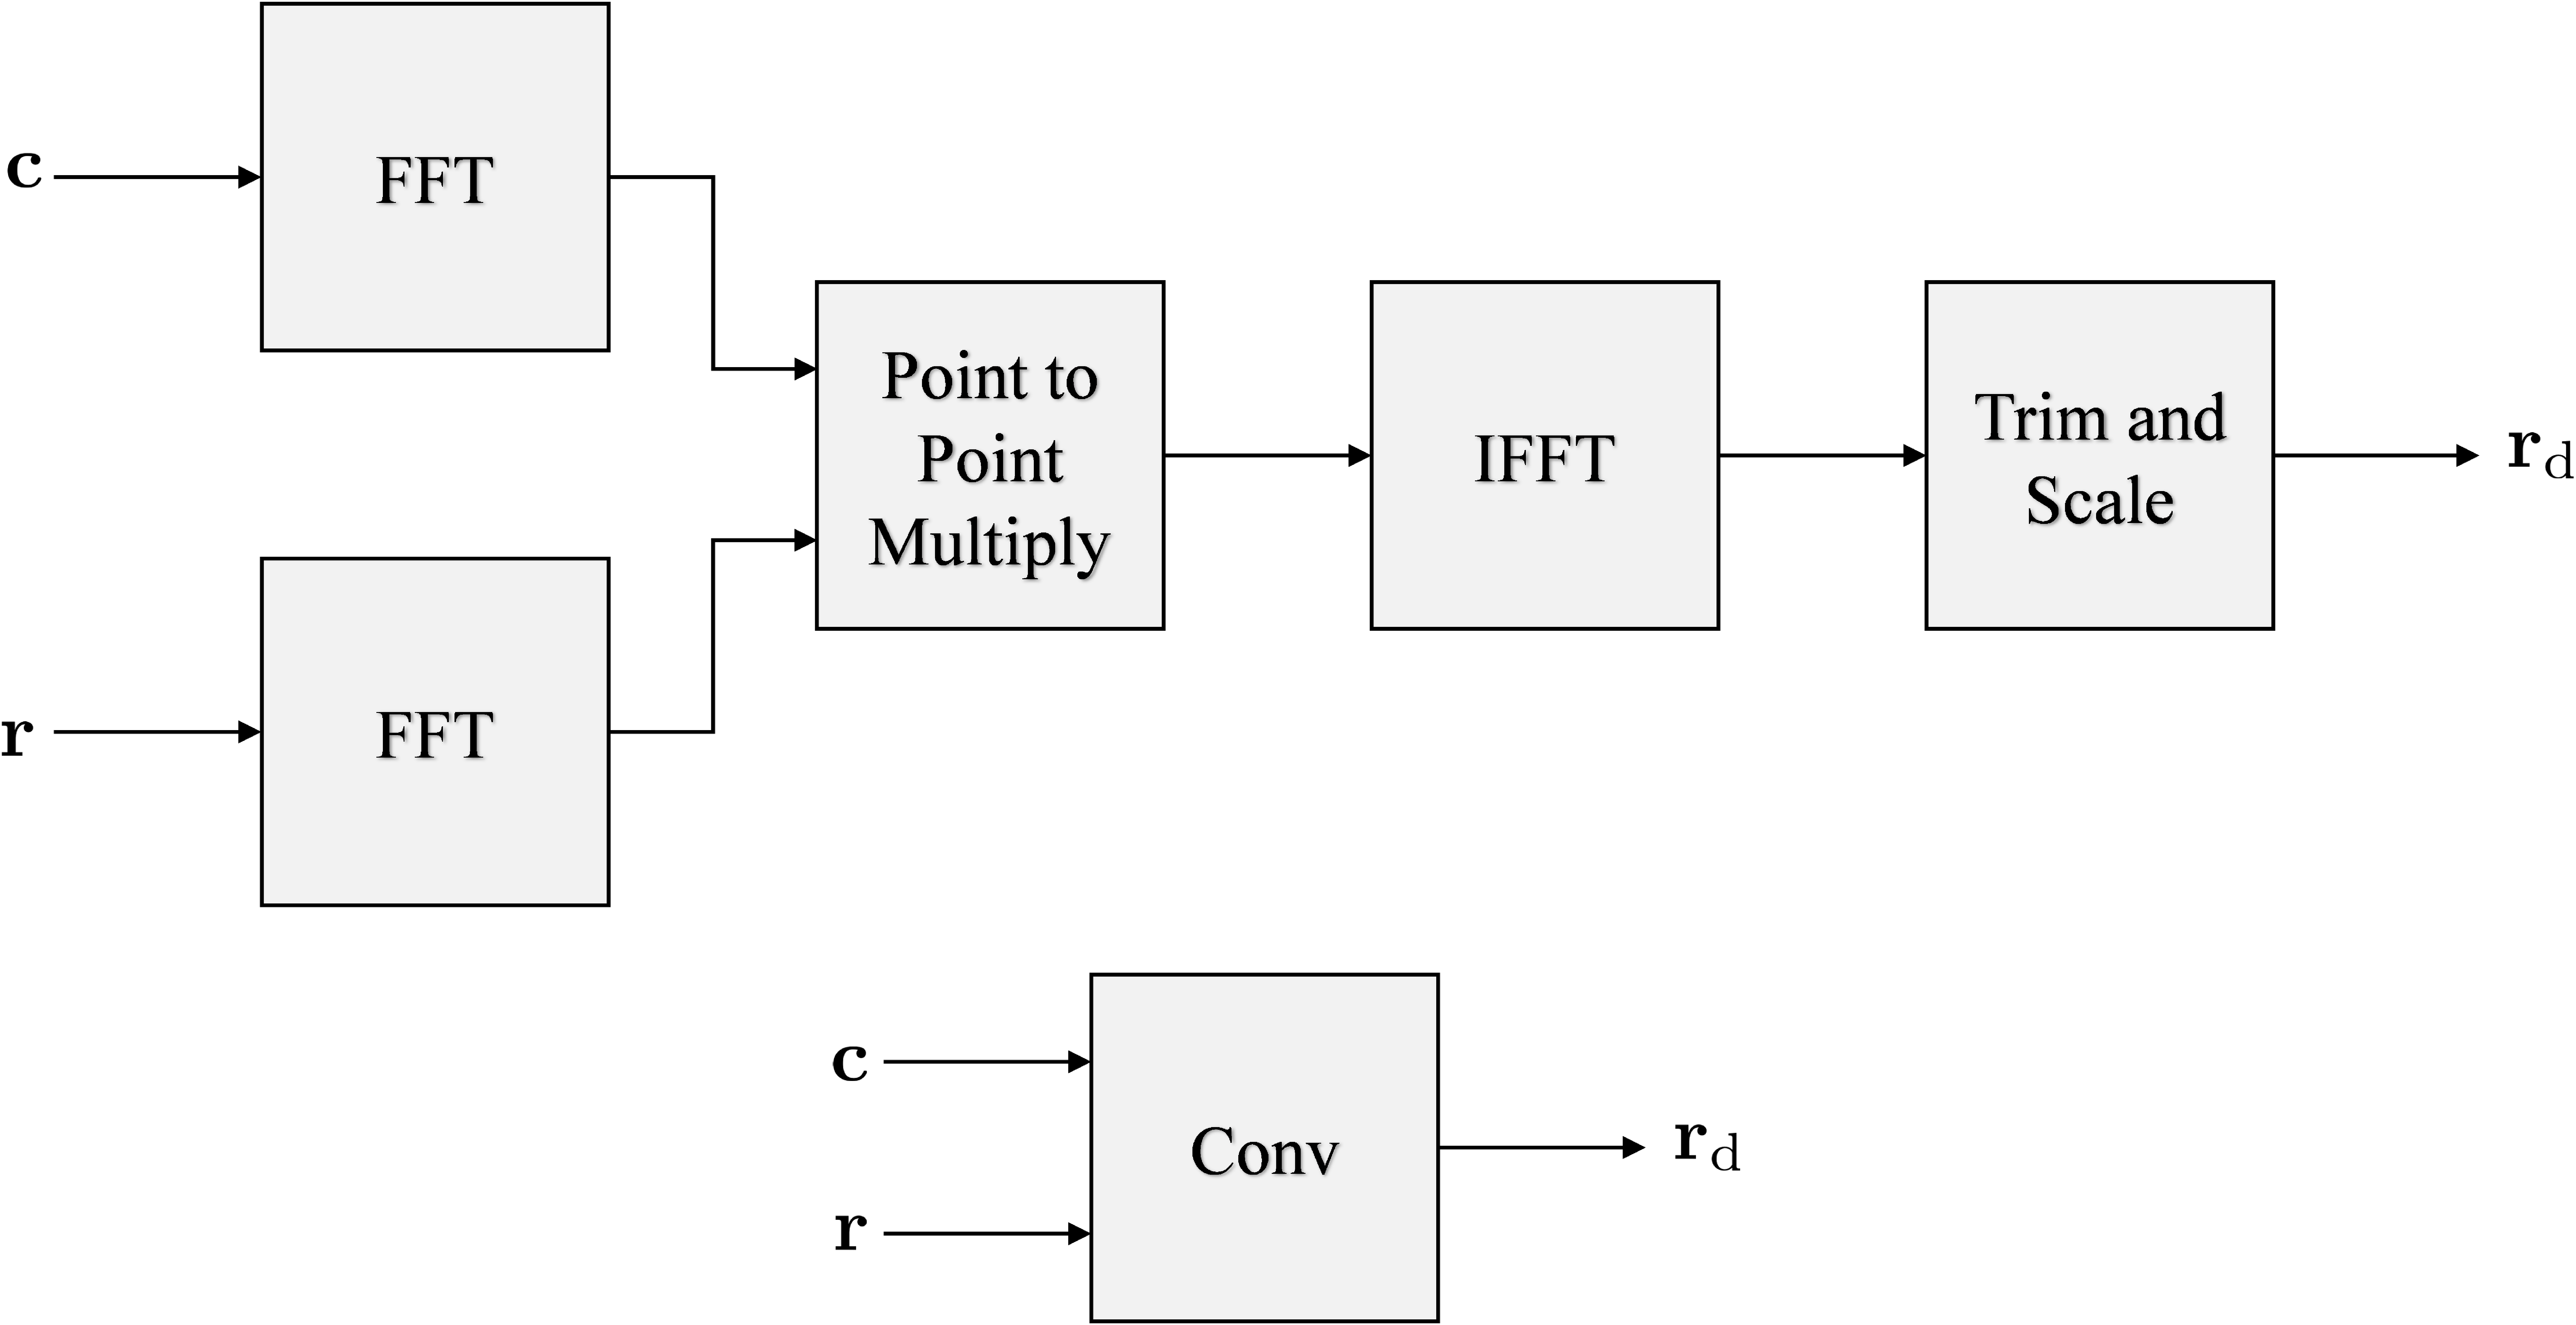
\includegraphics[width=9.27in/100*55]{figures/gpu_convolution/Conv2.pdf}
	\label{fig:Conv2}
	\caption{Convolution of vectors $\mathbf{c}$ and $\mathbf{r}$ block diagram simplified to one block marked Conv.}
\end{figure}
\begin{figure}
	\centering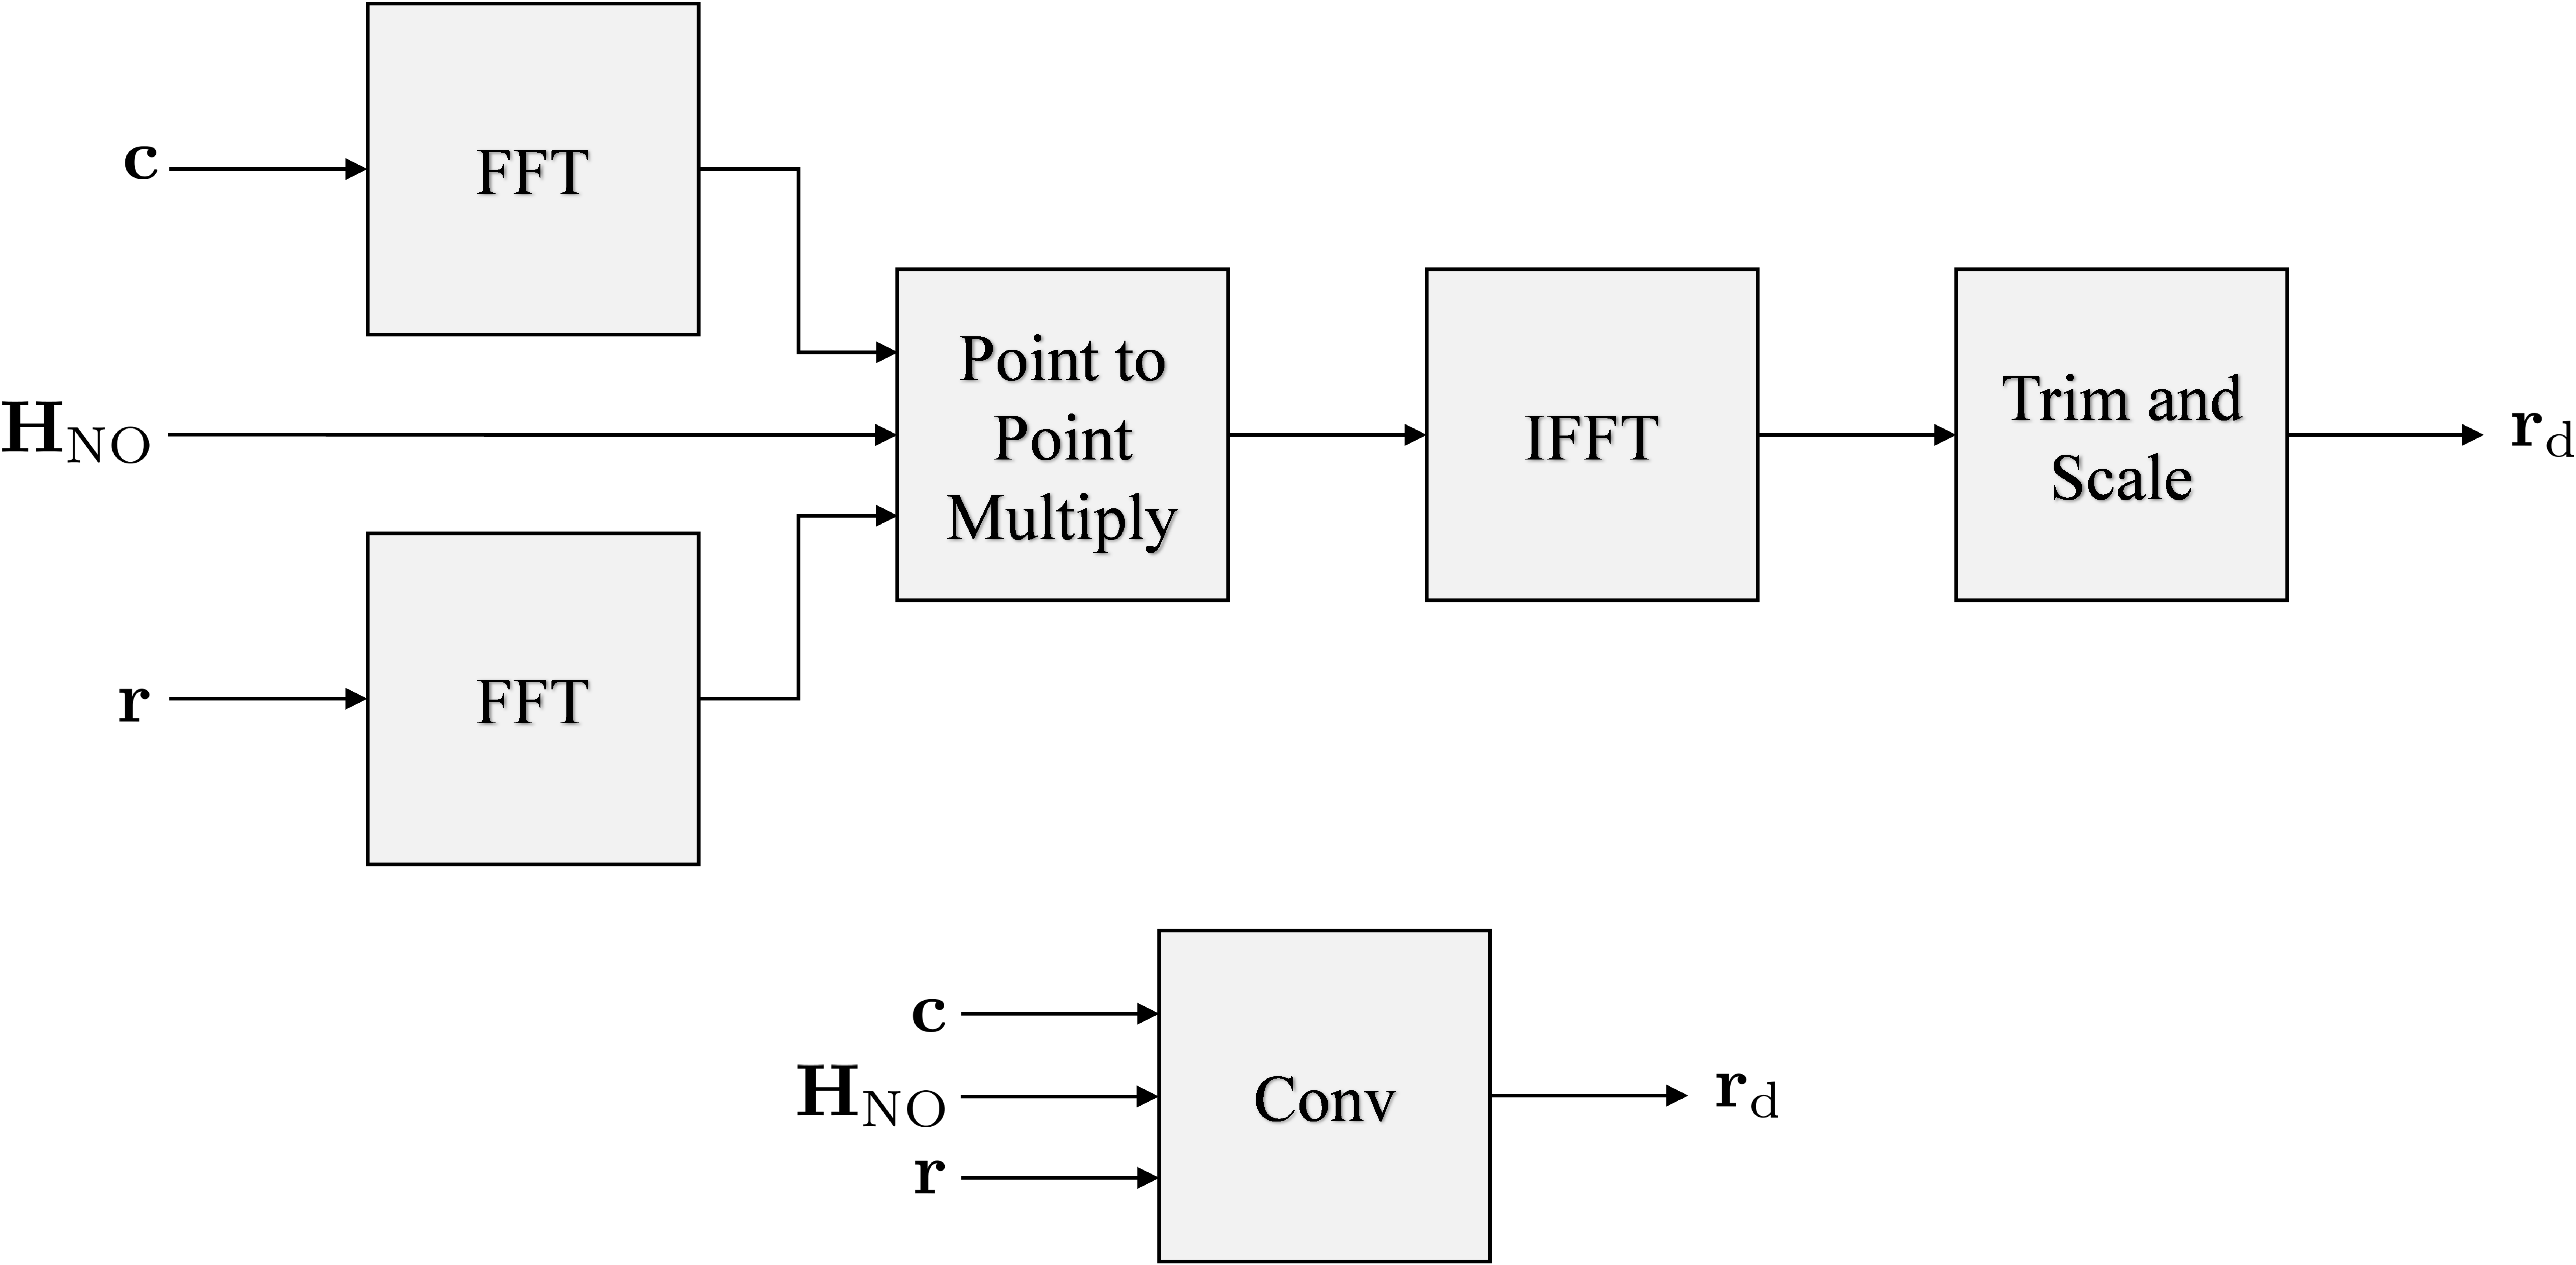
\includegraphics[width=9.27in/100*55]{figures/gpu_convolution/Conv3.pdf}
	\label{fig:Conv3}
	\caption{Convolution of vectors $\mathbf{c}$, $\mathbf{r}$ and $\mathbf{H}_{\text{NO}}$ block diagram simplified to one block marked Conv.}
\end{figure}


\section{Zero-Forcing and MMSE GPU Implementation}
The ZF and MMSE equalizer coefficient computations have exactly the same form as shown in Equations \ref{eq:c_ZF_solve} and \ref{eq:c_MMSE_solve}
\begin{equation}
\mathbf{R}_{\hat{h}} \mathbf{c}_\text{ZF} = \hat{\mathbf{h}}_{n_0}\\
\label{eq:ZF_gpuimp}
\end{equation}
\begin{equation}
\mathbf{R}_{\hat{h}w} \mathbf{c}_\text{MMSE} = \hat{\mathbf{h}}_{n_0}.
\label{eq:MMSE_gpuimp}
\end{equation}
The only difference is $\mathbf{R}_{\hat{h}}$ in ZF and $\mathbf{R}_{\hat{h}w}$ in MMSE.
Computing the ZF and MMSE equalizer coefficients is extremely computationally heavy.

It is possible to obtain the ZF and MMSE equalizer coefficients by computing the inverse of 
\begin{equation}
 \mathbf{c}_\text{ZF} = \mathbf{R}_{\hat{h}}^-1\hat{\mathbf{h}}_{n_0}
\label{eq:ZF_gpuimp}
\end{equation}
\begin{equation}
 \mathbf{c}_\text{MMSE} = \mathbf{R}_{\hat{h}w}^-1 \hat{\mathbf{h}}_{n_0}.
\label{eq:MMSE_gpuimp}
\end{equation}

Before solving Equation \ref{eq:ZF_gpuimp}, $\mathbf{R}_{\hat{h}}$ and $\hat{\mathbf{h}}_{n_0}$ need to be built and calculated given $\hat{\mathbf{h}}$.
The matrix $\mathbf{R}_{\hat{h}}$ requires the sample auto-correlation of the estimated channel $\mathbf{r}_{\hat{h}}$ and the time reversed channel and shifted channel $\hat{\mathbf{h}}_{n_0}$.

The vector $\hat{\mathbf{h}}_{n_0}$ is just the time reversed and conjugated estimated channel $\hat{\mathbf{h}}$. Building $\hat{\mathbf{h}}_{n_0}$ is trivial in the GPU and very little optimizing needs to be performed.
Computing the sample auto-correlation $\mathbf{r}_{\hat{h}}$ is done by implementing Equation \ref{eq:sample_autocorrelation} directly in one GPU kernel.
The computation of $\mathbf{r}_{\hat{h}}$ is very fast because the length of the channel estimate $L_{\text{ch}}$ is very short.

Section \ref{sec:zero-forcing} showed that $\mathbf{R}_{\hat{h}}$ is sparse because $r_{\hat{h}}(k)$ only has support on $-L_{\text{ch}} \leq k \leq L_{\text{ch}}$. 
To reduce computation time, the sparseness of $\mathbf{R}_{\hat{h}}$ will be leveraged. 
With out leveraging the sparse properties of $\mathbf{R}_{\hat{h}}$, even the mighty Tesla K40c cannot produce $\mathbf{c}_\text{ZF}$ in less than $500$ms.

The sparseness of $\mathbf{R}_{\hat{h}}$ is leveraged using a sparse solver function called ``cusolverSpCcsrqrsvBatched''.
cusolverSpCcsrqrsvBatched is a batched complex solver that leverages the sparse properties of $\mathbf{R}_{\hat{h}}$ by utilizing Compressed Row Storage (CRS) \cite{wiki:Sparse_matrix}.
The Compressed Row Storage reduces a large $186\times186$ matrix $\mathbf{R}_{\hat{h}}$ to a $12544$ element CSR matrix $\mathbf{R}_{\hat{h}\text{CRS}}$.
Before cusolverSpCcsrqrsvBatched can be called, the CSR matrix $\mathbf{R}_{\hat{h}\text{CRS}}$ has to be built using $\mathbf{r}_{\hat{h}}$.
An example of how to use the CUDA cusolverSp library can be found \cite{CUDA_toolkit_doc}.

Figure \ref{fig:blockZF} shows how the Zero-Forcing equalizer coefficients are implemented in the GPU.
\begin{figure}
	\centering\includegraphics[width=7.5in/100*55]{figures/eq_GPUimplementation/blockZF.pdf}
	\label{fig:blockZF}
	\caption{Block Diagram showing how the Zero-Forcing equalizer coefficients are implemented in the GPU.}
\end{figure}
The MMSE equalizer coefficients are computed nearly identically to ZF accept when calculating $\mathbf{R}_{\hat{h}w\text{CRS}}$, $\hat{\sigma}^2_w$ is added to the main diagonal elements.
\begin{figure}
	\centering\includegraphics[width=7.98in/100*55]{figures/eq_GPUimplementation/blockMMSE.pdf}
	\label{fig:blockMMSE}
	\caption{Block Diagram showing how the Minimum Mean Squared Error equalizer coefficients are implemented in the GPU.}
\end{figure}

Using cusolverSpCcsrqrsvBatched wasn't the only implementation researched.
Table \ref{tab:ZFMMSEtimingComparison} lists the algorithms researched and their respective execution times.
A custom GPU Levinson Recursion algorithm was built to leverage the Toeplitz structure of $\mathbf{R}_{\hat{h}}$ and $\mathbf{R}_{\hat{h}w}$ \cite[Chap. 5]{hayes:1996}. 
The Levinson Recursion algorithm initially showed promise when operating on real floats but when converted to complex data Levinson wasn't feasable.

Rather than solving for $\mathbf{c}_\text{ZF}$ or $\mathbf{c}_\text{MMSE}$, computing the full inverse of $\mathbf{R}_{\hat{h}}$ was researched using the cuBLAS LU Decomposition.
While using staying real time using cuBLAS was feasable, cusolverSp out performed cuBLAS by almost $2\times$.
\begin{table}
\caption{Defining start and stop lines for timing comparison in Listing \ref{code:convFun}.}
\begin{center}
\begin{tabular}{lll}
	\toprule
	Algorithm 			& Data type	& Execution Time (ms)	\\ \midrule
	Levinson Recursion 	& floats 	& 500 					\\
	Levinson Recursion 	& Complex 	& 2500 					\\
	LU Decomposition 	& Complex 	& 600				 	\\
	cuSolver			& Complex	& 355.96				\\
	\bottomrule
\end{tabular}
\end{center}
\label{tab:ZFMMSEtimingComparison}
\end{table}
%Jeff explains how CUDA solvers handle this equation.
%
%The ZF equalizer was studied in the PAQ Phase 1 Final Report in ~equation 324
%\begin{equation}
%\mathbf{c}_\text{ZF} = (\mathbf{H}^\dagger \mathbf{H})^{-1} \mathbf{H}^\dagger \mathbf{u}_{n_0}
%\label{eq:c_ZF_pinv}
%\end{equation}
%where $\mathbf{c}_\text{ZF}$ is a $L_{eq} \times 1$ vector of equalizer coefficients computed to invert the channel estimate $\hat{\mathbf{h}}$
%and $\mathbf{u}_{n_0}$ is the desired channel impulse response centered on $n0 = N_1+L_1+1$
%\begin{equation}
%\mathbf{u}_{n_0} = \begin{bmatrix} 0 \\ \vdots \\ 0 \\ 1 \\ 0 \\ \vdots \\ 0 \end{bmatrix}
%	\begin{matrix*}[l] \left. \vphantom{\begin{matrix} 0 \\ \vdots \\ 0 \end{matrix}} \right\}
%		\text{$n_0-1$ zeros}
%		\\ \\
%		\left. \vphantom{\begin{matrix} 0 \\ \vdots \\ 0 \end{matrix}} \right\}
%		\text{$N_1+N_2+L_1+L_2-n_0+1$ zeros}
%		\end{matrix*}.
%		\label{eq:un0_ZF}
%\end{equation}
%The $L_{eq}+N_1+N_2 \times L_{eq}$ convolution matrix $\mathbf{H}$ is built using the channel estimate $\hat{\mathbf{h}}$
%\begin{equation}
%\mathbf{H} = 
%		\begin{bmatrix}
%		h(-N_1)		&  			& 		 	&  			\\
%		h(-N_1+1) 	& h(-N_1)	& 		 	&  			\\
%		\vdots	 	& \vdots	& \ddots 	&  			\\
%		h(N_2)		& h(N_2-1) 	&  			& h(-N_1)  	\\
%		 			& h(N_2) 	&  			& h(-N_1+1) \\
%		 			&  	   		&  			& \vdots	\\
%		 			&  	   		&  			& h(N_2)	\\
%	\end{bmatrix}.
%\end{equation}
%The computation of the coefficients in Equation \eqref{eq:c_ZF_pinv} can be simplified in a couple of ways: First the matrix multiplication of $\mathbf{H}^\dagger$ and $\mathbf{H}$ is the autocorrelation matrix of the channel
%\begin{equation}
%\mathbf{R}_{\hat{h}} = 
%\mathbf{H}^\dagger \mathbf{H} = 
%		\begin{bmatrix}
%		r_{h}(0)		& r^\ast_{h}(1)	& \cdots 	& r^\ast_{h}(L_{eq}-1)  	\\
%		r_{h}(1) 		& r_{h}(0)		& \cdots 	& r^\ast_{h}(L_{eq}-2)  	\\
%		\vdots	 			& \vdots				& \ddots 	&  							\\
%		r_{h}(L_{eq}-1)	& r_{h}(L_{eq}-2)	& \cdots	& r_{h}(0)  			
%	\end{bmatrix}
%	\label{eq:R_h}
%\end{equation}
%where
%\begin{equation}
%r_{h}(k) = \sum_{n=-N_1}^{N_2} h(n) h^\ast(n-k).
%\end{equation}
%Second the matrix vector multiplication of $\mathbf{H}^\dagger$ and $\mathbf{u}_{n_0}$ is simply the $n_0$th row of $\mathbf{H}^\dagger$ or the conjugated $n_0$th column of $\mathbf{H}$.
%A new vector $\hat{\mathbf{h}}_{n_0}$ is defined by
%\begin{equation}
%\hat{\mathbf{h}}_{n_0} = \mathbf{H}^\dagger \mathbf{u}_{n_0} = 
%\begin{bmatrix} h(L_1) \\ \vdots \\ h(0) \\ \vdots \\ h(-L_2)  \end{bmatrix}.
%\label{eq:h_no}
%\end{equation}
%To simplify, Equations \eqref{eq:R_h} and \eqref{eq:h_no} are substituted into Equation \eqref{eq:c_ZF_pinv} resulting in 
%\begin{equation}
%\mathbf{c}_\text{ZF} = \mathbf{R}^{-1}_{h} \hat{\mathbf{h}}_{n_0}.
%\label{eq:c_ZF_R_h}
%\end{equation}
%
%Computing the inverse of $\mathbf{R}_{\hat{h}}$ is computationally heavy because an inverse is an $N^3$ operation.
%To avoid an inverse, $\mathbf{R}_{\hat{h}}$ is moved to the left side and $\mathbf{c}_\text{ZF}$ is found by solving a system of linear equations. 
%Note that $r_{h}(k)$ only has support on $-L_{ch} \leq k \leq L_{ch}$ making $\mathbf{R}_{\hat{h}}$ sparse or $\%63$ zeros.
%The sparseness of $\mathbf{R}_{\hat{h}}$ is leveraged to reduce computation drastically.
%The Zero-Forcing Equalizer coefficients are computed by solving
%\begin{equation}
%\mathbf{R}_{\hat{h}} \mathbf{c}_\text{ZF} = \hat{\mathbf{h}}_{n_0}.
%\label{eq:c_ZF_solve}
%\end{equation}


\section{Constant Modulus Algorithm GPU Implementation}
The Constant Modulus Algorithm (CMA) is quite a bit more complicated than all other equalizers.
CMA presented real challenges when implementing into a GPU.
The direct approach didn't allow for multiple iterations.
The more iterations CMA performed, the better CMA becomes becouse CMA is a steepest decent.

Each iteration of CMA uses the signal equalized by the most recent $\mathbf{c}_{\text{CMA}b}$
\begin{equation}
\mathbf{y} = \mathbf{r}*\mathbf{c}_{\text{CMA}b}.
\end{equation}
The element of the gradient $\nabla J(k)$ is calculate by convolving the $12672$ sample $\mathbf{z}$ and with the $12672$ sample $\rho$. 
Note that all other frequency domain convolutions in this Thesis are $\text{Nfft} = 2^{14}$, but the convolution length $12672+12672-1>2^{14}$. The FFTs in the computation of $\nabla J(k)$ are $\text{Nfft} = 2^{15}$ point FFTs.
The element  of the gradient vector $\nabla J(k)$ is calculated by
\begin{equation}
\nabla J(k) = \frac{1}{L_{pkt}} b(k), \quad -L_1 \leq k \leq L_2
\end{equation}
where
\begin{align}
b(n) &= \sum^{L_{pkt}-1}_{m=0} z(m) \rho(n-m) \nonumber \\
	 &= \sum^{L_{pkt}-1}_{m=0} z(m) r^\ast(m-n)
\end{align}
using convolution.
Once $\nabla J$ is calculated, the steepest decent algorithm is applied
\begin{equation}
\mathbf{c}_\text{CMA($b+1$)} = \mathbf{c}_\text{CMA($b$)}-\mu \nabla J.
\end{equation}
The goal of CMA is to perform as many iterations as possible.
Once done iterating, apply the last $\mathbf{c}_\text{CMA($b+1$)}$ to the received signal $\mathbf{r}$.

In Section \ref{sec:CMA}, the direct application of CMA was massaged into convolution.
Figure \ref{fig:blockCMA} shows a block diagram of how the CMA algorithm runs on the GPU.
\begin{figure}
	\centering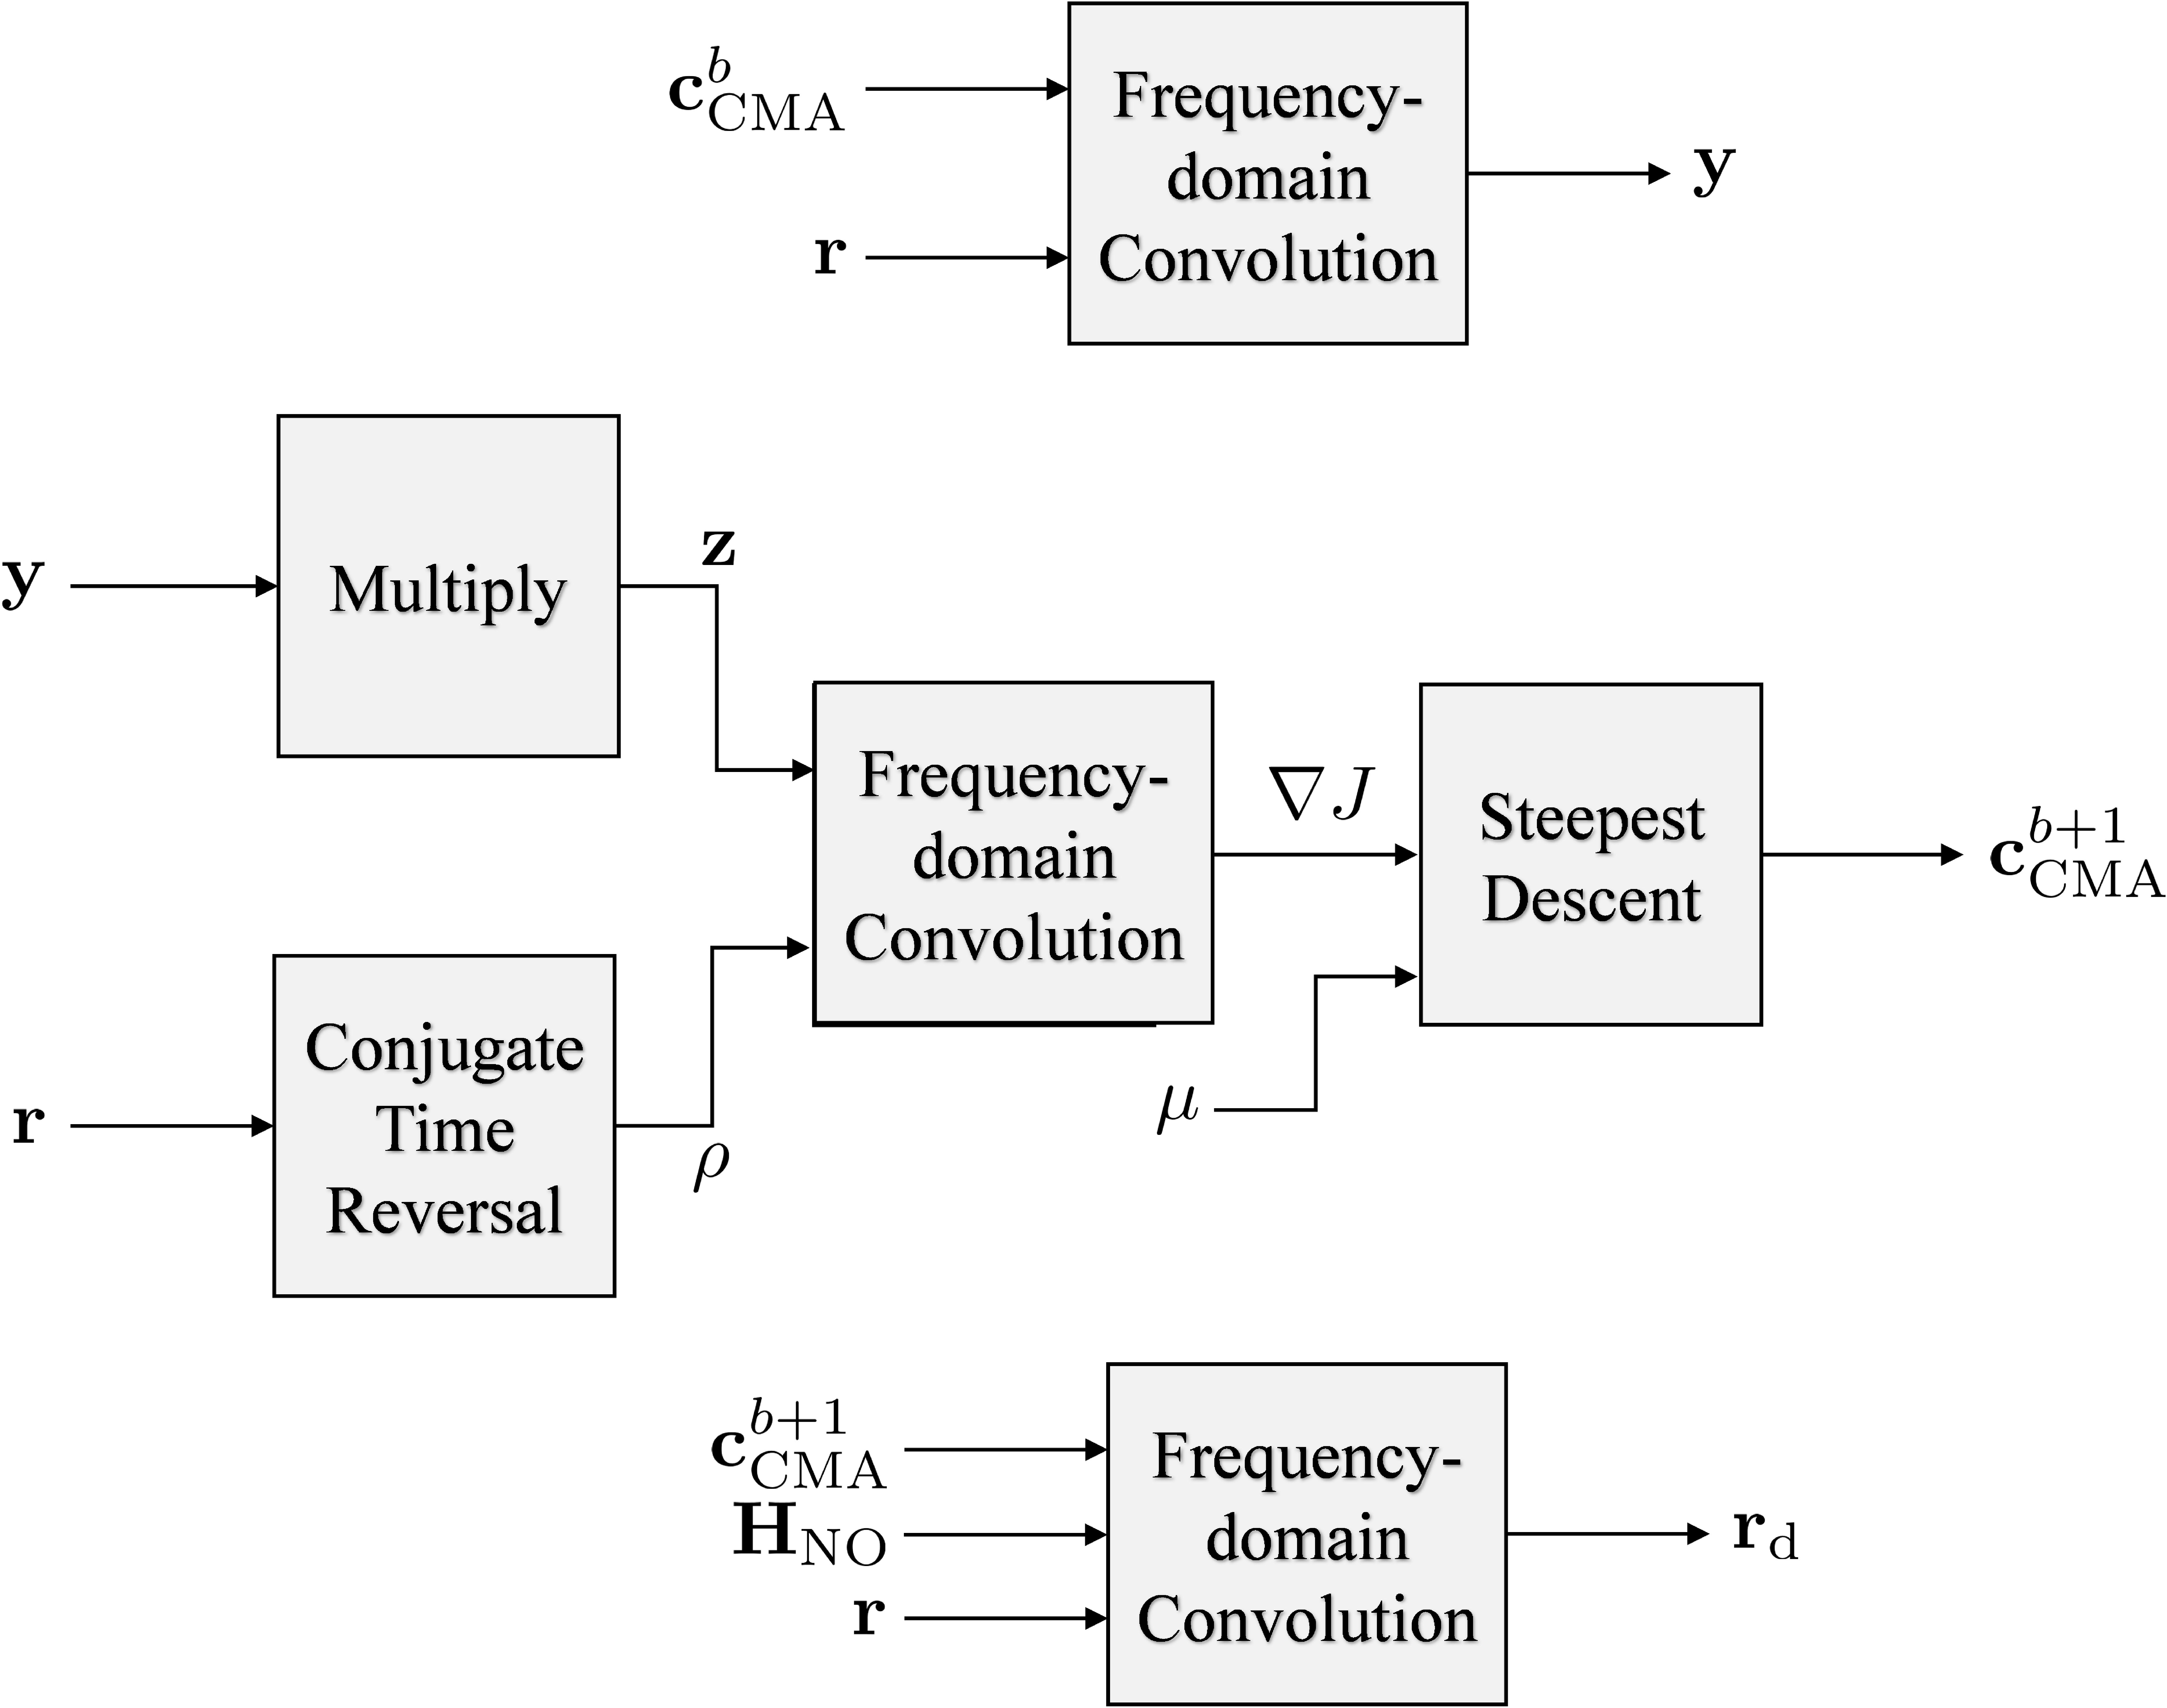
\includegraphics[width=8.34in/100*55]{figures/eq_GPUimplementation/blockCMA.pdf}
	\label{fig:blockCMA}
	\caption{Diagram showing the relationships between $z(n)$, $\rho(n)$ and $b(n)$.}
\end{figure}

The most computationally heavy part of CMA is computing $\nabla J(k)$.
Computing $\nabla J(k)$ directly is almost $5\times$ slower than using convolution.
The direct computation is done by performing a long $12672$ sample summation from Equation \ref{eq:delJ_direct_way}
\begin{equation}
\nabla J(k) = \frac{1}{L_{pkt}} \sum^{L_{pkt}-1}_{m=0}  z(m) r^\ast(m-k), \quad -L_1 \leq k \leq L_2.
\end{equation}
Long summations are slow in GPUs.
Table \ref{tab:CMAtimingComparison} lists the comparison on computing $\nabla J(k)$ verse using convolution.
\begin{table}
\caption{The gradient vector $\nabla J(k)$ can be computed using convolution or computed directly.}
\begin{center}
\begin{tabular}{lll}
	\toprule
	CMA	Iteration Algorithm			& Execution Time (ms)	\\ \midrule
	$\nabla J$ directly 			& 421.317				\\
	$\nabla J$ using convolution & 88.7743				\\
	\bottomrule
\end{tabular}
\end{center}
\label{tab:CMAtimingComparison}
\end{table}



\section{Frequency Domain Equalizer One and Two GPU Implementation}
The Frequency Domain Equalizers are by far the fastest and easiest to implement into GPUs.
The block diagram looks just like convolution accept that point to point multiply isn't a simple two or three point complex multiply.

Equation \ref{eq:FDE1} and is implemented directly in the GPU.
To save execution time, the FFT of the detection filter $\mathbf{H}_{\text{NO}}$ multiplied at the same time FDE1 is calculated 
\begin{equation}
R_\text{d1}(e^{j\omega_k}) = \frac{R(e^{j\omega_k}) \hat{H}^\ast(e^{j\omega_k}) H_{\text{NO}}(e^{j\omega_k})}  {|\hat{H}(e^{j\omega_k})|^2  +  \frac{1}{\hat{\sigma}^2_w}} \quad
\text{where} \;
\omega_k = \frac{2\pi}{L} \;
\text{for} \;
k=0,1,\cdots,L-1
\label{eq:FDE1_applied}
\end{equation}
\begin{equation}
R_\text{d2}(e^{j\omega_k}) = \frac{R(e^{j\omega_k}) \hat{H}^\ast(e^{j\omega_k}) H_{\text{NO}}(e^{j\omega_k})}  {|\hat{H}(e^{j\omega_k})|^2  +  \frac{\Psi(e^{j\omega_k})}{\hat{\sigma}^2_w}} \quad
\text{where} \;
\omega_k = \frac{2\pi}{L} \;
\text{for} \;
k=0,1,\cdots,L-1
\label{eq:FDE2_applied}
\end{equation}
where $R(e^{j\omega_k})$ and $R_\text{d}(e^{j\omega_k})$ is the FFT $\mathbf{r}$ and $\mathbf{r}_\text{d}$ 
at $\omega_k$.
\begin{table}
\caption{Defining start and stop lines for timing comparison in Listing \ref{code:convFun}.}
\begin{center}
\begin{tabular}{lll}
	\toprule
	Algorithm						& Execution Time (ms)	\\ \midrule
	Frequency Domain Equalizer One 	& 57.156				\\
	Frequency Domain Equalizer Two	& 58.841				\\
	\bottomrule
\end{tabular}
\end{center}
\label{tab:CMAtimingComparison}
\end{table}
Figures \ref{fig:blockFDE1} and \ref{fig:blockFDE2} show block diagrams of how FDE1 and FDE2 are implemented in the GPUs.
\begin{figure}
	\centering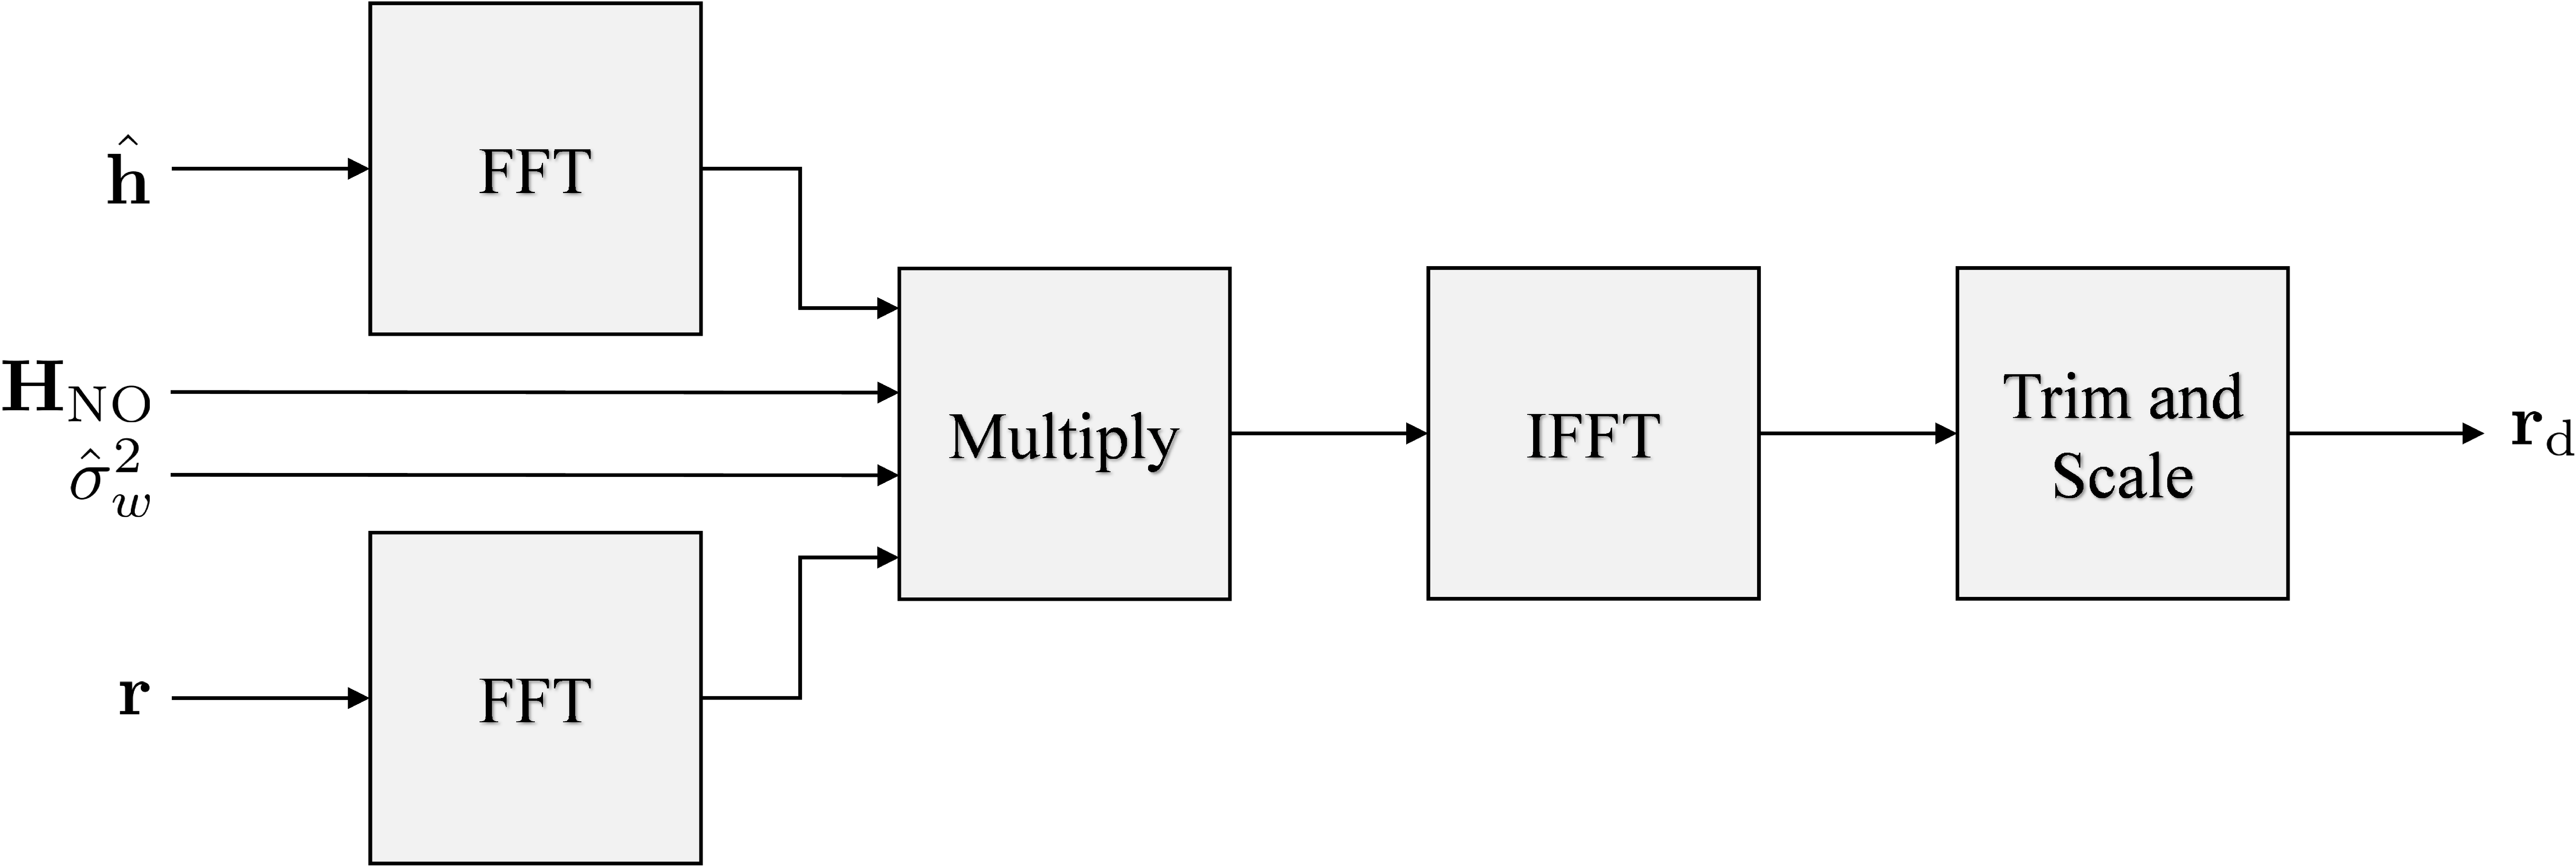
\includegraphics[width=9.73in/100*55]{figures/eq_GPUimplementation/blockFDE1.pdf}
	\label{fig:blockFDE1}
	\caption{Diagram showing Frequency Domain Equalizer One is implemented in the frequency domain in GPUs.}
\end{figure}
\begin{figure}
	\centering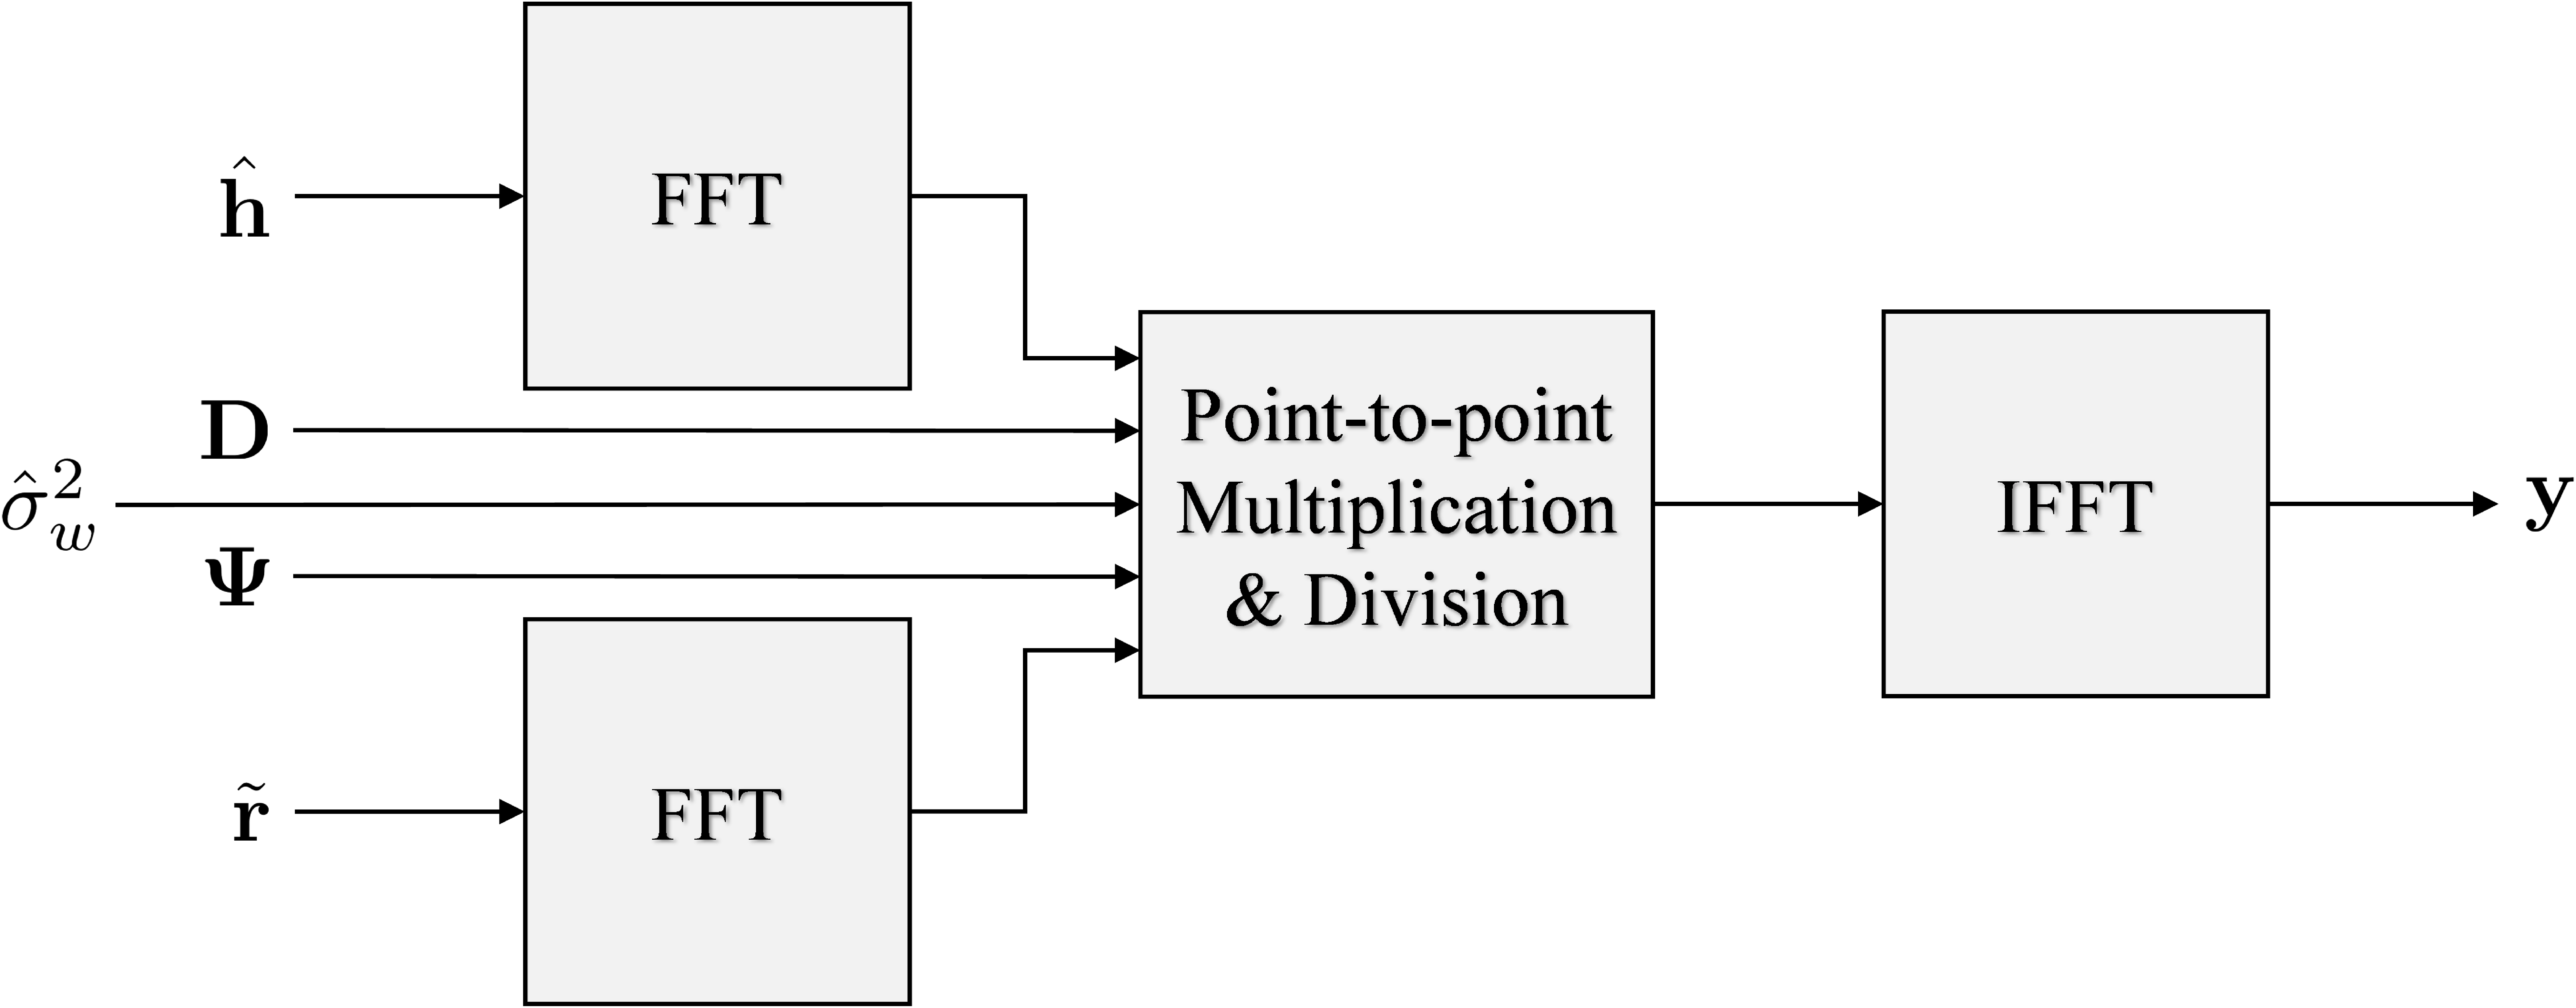
\includegraphics[width=10.03in/100*55]{figures/eq_GPUimplementation/blockFDE2.pdf}
	\label{fig:blockFDE2}
	\caption{Diagram showing Frequency Domain Equalizer Two is implemented in the frequency domain in GPUs.}
\end{figure}





